\section{An axiomatic network model}
\label{sect.network}

In this section, we incrementally work towards a formal definition of an asynchronous unreliable causal broadcast network.
This network model is useful because it gives us a realistic setting in which we can embed various replication algorithms, and prove that they guarantee strong eventual consistency in all possible executions of the network.
Our network model is defined using only six axioms, all of which are standard assumptions in the modelling of distributed systems, and which are satisfied by many systems in practice.
All theorems in this paper are derived from those axioms; in particular, we show that the causal delivery abstraction satisfies the strict partial ordering assumption of $\isa{hb-consistent}$ (Section~\ref{sect.happens.before}), allowing us to use the $\isa{convergence}$ theorem (Section~\ref{sect.ops.commute}) in locales that extend the network.

%TODO Martin to check that he is happy with the rest of this intro. Have we stated informally why we want to model an asynchronous unreliable causal broadcast network and what this means?
We start by assuming that all communication between nodes are sent as messages via the network and that these messages may be delayed, reordered, or lost entirely---an assumption that matches the behaviour of many networks in practice~\cite{Bailis:2014jx}.
Moreover, nodes or network links may fail at any time, and the non-faulty parts of the system need
to continue working in spite of such partial failures.

As motivated in the introduction, we do not wish to rely on a central server.
Rather, we aim to support scenarios in which subsets of
nodes can communicate with each other, but some are disconnected (\emph{partitioned}) from others.
It is possible to provide totally ordered delivery without a central server and thus obtain strong consistency; this abstraction is known as \emph{total order broadcast} or \emph{atomic broadcast} \cite{Cachin:2011wt,Defago:2004ji}. 
Unfortunately, it is expensive: it requires a quorum of nodes (typically a majority) to be reachable in order to make progress \cite{Chandra:1996cp}.
This is not an assumption we wish to make since, when nodes represent laptops or smartphones, it is likely that less than a majority of devices are online at any one time, and so any algorithm for total order broadcast would be stalled.

For example, consider some data shared between two users, each of whom has two devices. 
Each user may want to synchronise the data between their two devices using a local wireless link, even if they are temporarily disconnected from the internet, and re-synchronise with the other user when they are next online. 
In this scenario, strong consistency across both users could only be achieved by preventing users from making any offline updates; if updates are allowed, weaker consistency is inevitable \cite{Attiya:2015dm,Davidson:1985hv}.

We therefore use an \emph{asynchronous} network model, which means that we make no timing assumptions: messages sent over the network may suffer unbounded delays before they are delivered, or they may never arrive at all. 
Nodes may pause their execution for unbounded periods of time, or fail permanently \cite{Cachin:2011wt}. 
If a user makes updates while offline, and the device re-synchronises when it is next online, we can simply model that interaction as very large network delay.

%Although most practical systems have fairly low network delay and fairly brief execution pauses most of the time, the asynchronous model is a useful lower bound for the assumptions that a distributed algorithm may make. 
%Any algorithm that is proved correct under the assumptions of the asynchronous model is also guaranteed to be correct in a system that provides stronger guarantees, for example around timing and reliability.

If network interruptions between nodes last only for a finite time, every update can be eventually delivered to every non-failed node by re-sending messages until they arrive.
%Thus, all non-failed nodes will eventually deliver the same set of updates (although perhaps in a different order), and
%so strong eventual consistency will ensure that they all converge to an equivalent state. 
We can therefore assume that the network is \emph{unreliable}.
If nodes are partitioned from each other forever, they will not converge, but that is the case for any replication algorithm, since the network is assumed to be the only communication channel.
In such cases we assume that the node has failed.

\subsection{Modelling a distributed system}

We begin by modelling a distributed system as an arbitrary, unbounded number of nodes.
At the most abstract level, we do not assume anything about their communication pattern---we assume only that each node is uniquely identified by a natural number, and that the flow of execution at each node consists of a finite, totally ordered sequence of execution steps (events).
We call that sequence of events at node $i$ the \emph{history} of that node.
For convenience, we assume that every event or execution step is unique within a node's history; this assumption is standard in the modelling of distributed systems \cite{Cachin:2011wt} and can easily be implemented by attaching a sequence number, timestamp, or other unique identifier to each event.
This system model can be expressed in Isabelle as follows:
\vspace{0.375em}
\begin{isabellebody}
\ \ \ \ \ \ \ \ \isacommand{locale} node{\isacharunderscore}histories\ {\isacharequal}\ \isanewline
\ \ \ \ \ \ \ \ \ \ \isakeyword{fixes}\ history\ {\isacharcolon}{\isacharcolon}\ {\isachardoublequoteopen}nat\ {\isasymRightarrow}\ {\isacharprime}a\ list{\isachardoublequoteclose}\ \isakeyword{assumes}\ histories{\isacharunderscore}distinct{\isacharcolon}\ {\isachardoublequoteopen}distinct\ {\isacharparenleft}history\ i{\isacharparenright}{\isachardoublequoteclose}
\end{isabellebody}
\vspace{0.375em}
Here, the history of a node $\isa{i}$ is obtained by using a function fixed by the local theory, $\isa{history}$.
The history is simply a list of events, and each event is modelled as an abstract type variable---here we use $\isa{{\isacharprime}a}$.
The $\isa{distinct}$ predicate is an Isabelle/HOL library function that asserts that a list contains no duplicate elements, up to equality.
Note that we make no assumption about the number of nodes in the system, which allows us to model systems in which nodes join and leave the network over time.
A node that does not exist is simply modelled by an empty list of events.

Isabelle lists are finite, and therefore so is a node's history.
At the end of a node's history, we assume that a node has either failed or successfully terminated.
In this model, a node failure is permanent, and is modelled by the absence of any further events in its history (there is no explicit failure event).
This \emph{crash-stop} abstraction is commonly used by distributed algorithms \cite{Cachin:2011wt}.

Within the $\isa{node{\isacharunderscore}histories}$ locale we may define when one event \emph{comes before} another at one particular node.
We write $\isa{x} \sqsubset^\isa{i} \isa{y}$ whenever event $\isa{x}$ comes before event $\isa{y}$ in the history of node $\isa{i}$.
More formally, $\isa{x} \sqsubset^\isa{i} \isa{y}$ whenever there exist lists $\isa{xs}$, $\isa{ys}$, and $\isa{zs}$ such that $\isa{xs}\mathbin{@}[\isa{x}]\mathbin{@}\isa{ys}\mathbin{@}[\isa{y}]\mathbin{@}\isa{zs} = \isa{history\ i}$.

\subsection{An asynchronous broadcast network}

We now extend the $\isa{node-histories}$ locale by defining how nodes can communicate.
We specialise $\isacharprime\isa{a}$ to be one of two kinds of event: either \emph{broadcast} or \emph{deliver}.
(They could equivalently be called \emph{send} and \emph{receive}, but we stick to the conventional distributed systems terminology.)
Each event contains a message of some abstract type $\isacharprime\isa{msg}$:
\vspace{0.375em}
\begin{isabellebody}
\ \ \ \ \ \ \ \ \isacommand{datatype} {\isacharprime}msg\ event\ {\isacharequal}\ Broadcast\ {\isacharprime}msg\ {\isacharbar}\ Deliver\ {\isacharprime}msg
\end{isabellebody}
\vspace{0.375em}
Intuitively, a node can be regarded as a deterministic state machine where each state transition corresponds to a broadcast or deliver event.
We assume that users may query the state of any node at any time, and such queries need not be reflected as events, since they neither modify the node state nor send or receive any messages.

We then define a new locale $\isa{network}$ containing three axioms that define how broadcast and deliver events may interact, and these axioms define the properties of our network model.
Since $\isa{network}$ is an extension of $\isa{node-histories}$, the aforementioned definitions of $\isa{history}$ and $\sqsubset^\isa{i}$ are available for use in the $\isa{network}$ axioms:
\vspace{0.375em}
\begin{isabellebody}
\ \ \ \ \ \ \ \ \isacommand{locale}\ network\ {\isacharequal}\ node{\isacharunderscore}histories\ history\ \isakeyword{for}\ history\ {\isacharcolon}{\isacharcolon}\ {\isachardoublequoteopen}nat\ {\isasymRightarrow}\ {\isacharprime}msg\ event\ list{\isachardoublequoteclose}\ {\isacharplus}\isanewline
\ \ \ \ \ \ \ \ \ \ \isakeyword{fixes}\ msg{\isacharunderscore}id\ {\isacharcolon}{\isacharcolon}\ {\isachardoublequoteopen}{\isacharprime}msg\ {\isasymRightarrow}\ {\isacharprime}msgid{\isachardoublequoteclose}\isanewline
\ \ \ \ \ \ \ \ \ \ \isakeyword{assumes}\ delivery{\isacharunderscore}has{\isacharunderscore}a{\isacharunderscore}cause{\isacharcolon}\ {\isachardoublequoteopen}Deliver\ m\ {\isasymin}\ set\ {\isacharparenleft}history\ i{\isacharparenright}\ {\isasymLongrightarrow}\ {\isasymexists}j{\isachardot}\ Broadcast\ m\ {\isasymin}\ set\ {\isacharparenleft}history\ j{\isacharparenright}{\isachardoublequoteclose}\isanewline
\ \ \ \ \ \ \ \ \ \ \ \ \ \ \isakeyword{and}\ deliver{\isacharunderscore}locally{\isacharcolon}\ {\isachardoublequoteopen}Broadcast\ m\ {\isasymin}\ set\ {\isacharparenleft}history\ i{\isacharparenright}\ {\isasymLongrightarrow}\ Broadcast\ m\ {\isasymsqsubset}\isactrlsup i\ Deliver\ m{\isachardoublequoteclose}\isanewline
\ \ \ \ \ \ \ \ \ \ \ \ \ \ \isakeyword{and}\ msg{\isacharunderscore}id{\isacharunderscore}unique{\isacharcolon}\ {\isachardoublequoteopen}Broadcast\ m{\isadigit{1}}\ {\isasymin}\ set\ {\isacharparenleft}history\ i{\isacharparenright}\ {\isasymLongrightarrow}\ Broadcast\ m{\isadigit{2}}\ {\isasymin}\ set\ {\isacharparenleft}history\ j{\isacharparenright}\ {\isasymLongrightarrow}\isanewline
\ \ \ \ \ \ \ \ \ \ \ \ \ \ \ \ \ \ \ \ \ \ \ \ \ \ \ \ msg{\isacharunderscore}id\ m{\isadigit{1}}\ {\isacharequal}\ msg{\isacharunderscore}id\ m{\isadigit{2}}\ {\isasymLongrightarrow}\ i\ {\isacharequal}\ j\ {\isasymand}\ m{\isadigit{1}}\ {\isacharequal}\ m{\isadigit{2}}{\isachardoublequoteclose}
\end{isabellebody}
\vspace{0.375em}
The axioms can be understood as follows:
\begin{description}
    \item[delivery-has-a-cause:] If some message $\isa{m}$ was delivered at some node, then there exists some node on which $\isa{m}$ was broadcast.
        With this axiom, we assert that messages are not created ``out of thin air'' by the network itself, and that the only source of messages are the nodes.
    \item[deliver-locally:] If a node broadcasts some message $\isa{m}$, then the same node must subsequently also deliver $\isa{m}$ to itself.
        Since $\isa{m}$ does not actually travel over the network, this local delivery is always possible, even if the network is interrupted.
        Local delivery may seem redundant, since the effect of the delivery could also be implemented by the broadcast event itself; however, it is standard practice in the description of broadcast protocols that the sender of a message also sends it to itself, since this property simplifies the definition of algorithms built on top of the broadcast abstraction \cite{Cachin:2011wt}.
    \item[msg-id-unique:] We do not assume that the message type $\isacharprime\isa{msg}$ has any particular structure; we only assume the existence of a function $\isa{msg-id} \mathbin{\isacharcolon\isacharcolon} \isacharprime\isa{msg} \mathbin{\isasymRightarrow} \isacharprime\isa{msgid}$ that maps every message to some globally unique identifier of type $\isacharprime\isa{msgid}$.
        We assert this uniqueness by stating that if $\isa{m1}$ and $\isa{m2}$ are any two messages broadcast by any two nodes, and their $\isa{msg-id}$s are the same, then they were in fact broadcast by the same node and the two messages are identical. 
        In practice, these globally unique IDs can by implemented using unique node identifiers, sequence numbers, timestamps, or random numbers.
\end{description}

In addition, the $\isa{network}$ locale inherits the $\isa{histories-distinct}$ axiom from the parent locale $\isa{node-histories}$.
Many other properties that we require can be deduced as lemmas from these axioms.
For example, we can prove that for every message message that is delivered by some node, there is exactly one broadcast event (on the same or some other node) that created the message.
Also, due to the $\isa{histories-distinct}$ axiom we know that the same message is not delivered more than once, an aspect that can easily be implemented in practical systems by deduplicating messages based on their unique ID.

Note, however, that we are not making any assumptions about the reliability or the ordering of messages.
If one node broadcasts a message, it \emph{may} be delivered by other nodes, but we do not state if or when that will happen.
Messages may be arbitrarily delayed, reordered, or even lost entirely.
It is even acceptable for a node to never deliver any messages besides those it broadcasts itself, modelling a node that is permanently disconnected from the network.

\subsection{Causally ordered delivery}

As discussed in Section~\ref{sect.happens.before}, some replication algorithms require that some operations be applied in a particular order because the later operation has a causal dependency on the earlier one.
We previously characterised these dependencies using the \emph{happens-before} relation $\prec$, which we required to be a strict partial order, but otherwise kept abstract.
In Section~\ref{sect.abstract.convergence} we reasoned about the order of \emph{operations}, but in a network we work with \emph{messages}.
We will connect operations and messages in Section~\ref{sect.network.ops}; for now we will define a particular instance of the ordering relation $\prec$ on messages, and prove that it satisfies the requirements of a strict partial order.

We do not use physical time (such as UTC) to define the order of messages, since reliance on physical time is often problematic in distributed systems \cite{Sheehy:2015jm}.
Instead, we say that a message $\isa{m1}$ happens before another message $\isa{m2}$ if the node that generated $\isa{m2}$ ``knew about'' $\isa{m1}$ at the time $\isa{m2}$ was generated.
More precisely, based on the well-known definition by \citet{Lamport:1978jq}, we say that $\isa{m1}\prec\isa{m2}$ if any of the following is true:
\begin{enumerate}
\item $\isa{m1}$ and $\isa{m2}$ were broadcast by the same node, and $\isa{m1}$ was broadcast before $\isa{m2}$.
\item The node that broadcast $\isa{m2}$ had delivered $\isa{m1}$ before it broadcast $\isa{m2}$.
\item There exists some operation $\isa{m3}$ such that $\isa{m1} \prec \isa{m3}$ and $\isa{m3} \prec \isa{m2}$.
\end{enumerate}

\ifextended
\begin{figure}
\centering
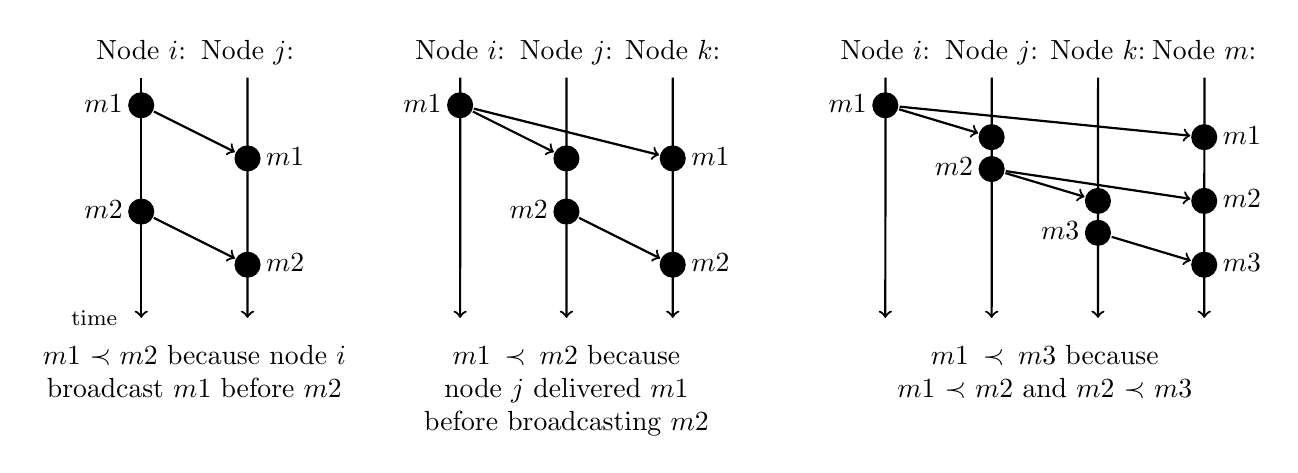
\begin{tikzpicture}[auto,scale=1.35]

\tikzstyle{event}=[circle,fill,minimum size=2pt]
\tikzstyle{label}=[text height=8pt,text depth=3pt]
\tikzstyle{leftlabel}=[label,left=3pt]
\tikzstyle{rightlabel}=[label,right=3pt]
\tikzstyle{every path}=[thick,->]
\tikzstyle{caption}=[text width=4cm,text centered,text height=8pt,below=5pt]

\node [label] (i1name) at (0,2.5) {Node $i$:};
\node [label] (j1name) at (1,2.5) {Node $j$:};
\node [event] (op1send) at (0,2.0) {};
\node [event] (op1recv) at (1,1.5) {};
\node [event] (op2send) at (0,1.0) {};
\node [event] (op2recv) at (1,0.5) {};
\node [leftlabel]  at (0,2.0) {$\isa{m1}$};
\node [rightlabel] at (1,1.5) {$\isa{m1}$};
\node [leftlabel]  at (0,1.0) {$\isa{m2}$};
\node [rightlabel] at (1,0.5) {$\isa{m2}$};
\draw (i1name) -- (0,0) node [left=5pt,at end] {\footnotesize time};
\draw (j1name) -- (1,0);
\draw (op1send) -- (op1recv);
\draw (op2send) -- (op2recv);
\node [caption] at (0.5,0) {
    $\isa{m1} \prec \isa{m2}$
    because node $i$ broadcast $\isa{m1}$ before $\isa{m2}$
};

\node [label] (i2name) at (3,2.5) {Node $i$:};
\node [label] (j2name) at (4,2.5) {Node $j$:};
\node [label] (k2name) at (5,2.5) {Node $k$:};
\node [event] (op3send) at (3,2.0) {};
\node [event] (op3recj) at (4,1.5) {};
\node [event] (op3reck) at (5,1.5) {};
\node [event] (op4send) at (4,1.0) {};
\node [event] (op4reck) at (5,0.5) {};
\node [leftlabel]  at (3,2.0) {$\isa{m1}$};
\node [rightlabel] at (5,1.5) {$\isa{m1}$};
\node [leftlabel]  at (4,1.0) {$\isa{m2}$};
\node [rightlabel] at (5,0.5) {$\isa{m2}$};
\draw (i2name) -- (3,0);
\draw (j2name) -- (4,0);
\draw (k2name) -- (5,0);
\draw (op3send) -- (op3recj);
\draw (op3send) -- (op3reck);
\draw (op4send) -- (op4reck);
\node [caption] at (4.0,0) {
    $\isa{m1} \prec \isa{m2}$
    because node $j$ delivered $\isa{m1}$ before broadcasting $\isa{m2}$
};

\node [label] (i3name) at  (7,2.5) {Node $i$:};
\node [label] (j3name) at  (8,2.5) {Node $j$:};
\node [label] (k3name) at  (9,2.5) {Node $k$:};
\node [label] (m3name) at (10,2.5) {Node $m$:};
\node [event] (op5send) at  (7,2.0) {};
\node [event] (op5recj) at  (8,1.7) {};
\node [event] (op5recm) at (10,1.7) {};
\node [event] (op6send) at  (8,1.4) {};
\node [event] (op6reck) at  (9,1.1) {};
\node [event] (op6recm) at (10,1.1) {};
\node [event] (op7send) at  (9,0.8) {};
\node [event] (op7recm) at (10,0.5) {};
\node [leftlabel]  at  (7,2.0) {$\isa{m1}$};
\node [rightlabel] at (10,1.7) {$\isa{m1}$};
\node [leftlabel]  at  (8,1.4) {$\isa{m2}$};
\node [rightlabel] at (10,1.1) {$\isa{m2}$};
\node [leftlabel]  at  (9,0.8) {$\isa{m3}$};
\node [rightlabel] at (10,0.5) {$\isa{m3}$};
\draw (i3name) -- (7,0);
\draw (j3name) -- (8,0);
\draw (k3name) -- (9,0);
\draw (m3name) -- (10,0);
\draw (op5send) -- (op5recj);
\draw (op5send) -- (op5recm);
\draw (op6send) -- (op6reck);
\draw (op6send) -- (op6recm);
\draw (op7send) -- (op7recm);
\node [caption] at (8.5,0) {
    $\isa{m1} \prec \isa{m3}$ because
    $\isa{m1} \prec \isa{m2}$ and
    $\isa{m2} \prec \isa{m3}$
};

\end{tikzpicture}

\caption{Illustrating the three conditions under which we consider one message to ``happen before'' another.}\label{fig.happens-before}
\end{figure}
The three cases are illustrated in Figure~\ref{fig.happens-before}.
\fi
This verbal definition translates directly into Isabelle syntax:
\vspace{0.375em}
\begin{isabellebody}
\ \ \ \ \ \ \ \ \isacommand{inductive} {\isacharparenleft}\isakeyword{in}\ network{\isacharparenright}\ hb\ {\isacharcolon}{\isacharcolon}\ {\isachardoublequoteopen}{\isacharprime}msg\ {\isasymRightarrow}\ {\isacharprime}msg\ {\isasymRightarrow}\ bool{\isachardoublequoteclose}\ \isakeyword{where}\isanewline
\ \ \ \ \ \ \ \ \ \ {\isachardoublequoteopen}{\isasymlbrakk}\ Broadcast\ m{\isadigit{1}}\ {\isasymsqsubset}\isactrlsup i\ Broadcast\ m{\isadigit{2}}\ {\isasymrbrakk}\ {\isasymLongrightarrow}\ m{\isadigit{1}}\ $\prec$\ m{\isadigit{2}}{\isachardoublequoteclose}\ {\isacharbar}\isanewline
\ \ \ \ \ \ \ \ \ \ {\isachardoublequoteopen}{\isasymlbrakk}\ Deliver\ m{\isadigit{1}}\ {\isasymsqsubset}\isactrlsup i\ Broadcast\ m{\isadigit{2}}\ {\isasymrbrakk}\ {\isasymLongrightarrow}\ m{\isadigit{1}}\ $\prec$\ m{\isadigit{2}}{\isachardoublequoteclose}\ {\isacharbar}\isanewline
\ \ \ \ \ \ \ \ \ \ {\isachardoublequoteopen}{\isasymlbrakk}\ m{\isadigit{1}}\ $\prec$\  m{\isadigit{2}}{\isacharsemicolon}\ m{\isadigit{2}}\ $\prec$\ m{\isadigit{3}}\ {\isasymrbrakk}\ {\isasymLongrightarrow}\ m{\isadigit{1}}\ $\prec$\ m{\isadigit{3}}{\isachardoublequoteclose}
\end{isabellebody}
\vspace{0.375em}
Given this definition, we define a restricted variant of our broadcast network model by extending the $\isa{network}$ locale.
In addition to the existing $\isa{network}$ axioms, we require that if there are any happens-before dependencies between messages, they must be delivered in that order.
Concurrent messages may be delivered in any order.
We express this requirement as follows:
\vspace{0.375em}
\begin{isabellebody}
\ \ \ \ \ \ \ \ \isacommand{locale} causal{\isacharunderscore}network\ {\isacharequal}\ network\ {\isacharplus}\isanewline
\ \ \ \ \ \ \ \ \ \ \ \isakeyword{assumes}\ causal{\isacharunderscore}delivery{\isacharcolon}\ {\isachardoublequoteopen}Deliver\ m{\isadigit{2}}\ {\isasymin}\ set\ {\isacharparenleft}history\ i{\isacharparenright}\ {\isasymLongrightarrow}\ m{\isadigit{1}}\ $\prec$\ m{\isadigit{2}}\ {\isasymLongrightarrow}\ Deliver\ m{\isadigit{1}}\ {\isasymsqsubset}\isactrlsup i\ Deliver\ m{\isadigit{2}}{\isachardoublequoteclose}
\end{isabellebody}
\vspace{0.375em}
The $\isa{causal-delivery}$ axiom does not strengthen the reliability assumptions of the network: only in the case where some message $\isa{m2}$ is delivered, it requires that any causally preceding messages are delivered first.
It is still possible for some message never to be delivered.
The abstraction defined by this locale is known as \emph{causal broadcast}, and it is typically implemented in network protocols using vector timestamps \cite{Schwarz:1994gl,Fidge:1988tv,Raynal:1996jl}.
As these protocols are widely known and well understood, we leave them out of scope for this paper.

\subsection{Using operations in the network}\label{sect.network.ops}

We can now include the convergence theorem into our network model by further extending the $\isa{causal-network}$ locale.
In the new locale $\isa{network-with-ops}$ we do not assume any additional axioms---we only assume the existence of an interpretation function (see Section~\ref{sect.ops.interpretation}) and some fixed initial state:
\vspace{0.375em}
\begin{isabellebody}
\ \ \ \ \ \ \ \ \isacommand{locale}\ network{\isacharunderscore}with{\isacharunderscore}ops\ {\isacharequal}\ causal{\isacharunderscore}network\ history\isanewline
\ \ \ \ \ \ \ \ \ \ \isakeyword{for}\ history\ {\isacharcolon}{\isacharcolon}\ {\isachardoublequoteopen}nat\ {\isasymRightarrow}\ {\isacharprime}msg\ event\ list{\isachardoublequoteclose}\ {\isacharplus}\isanewline
\ \ \ \ \ \ \ \ \ \ \isakeyword{fixes}\ interp\ {\isacharcolon}{\isacharcolon}\ {\isachardoublequoteopen}{\isacharprime}msg\ {\isasymRightarrow}\ {\isacharprime}state\ {\isasymrightharpoonup}\ {\isacharprime}state{\isachardoublequoteclose}\isanewline
\ \ \ \ \ \ \ \ \ \ \isakeyword{and}\ initial{\isacharunderscore}state\ {\isacharcolon}{\isacharcolon}\ {\isachardoublequoteopen}{\isacharprime}state{\isachardoublequoteclose}
\end{isabellebody}
\vspace{0.375em}
We have proved that the happens-before relation $\prec$ defined in the network is a strict partial order, so it meets the requirements of the $\isa{happens-before}$ locale.
Moreover, we can prove that the sequence of message deliveries at any node is consistent with $\prec$, that is, it satisfies the definition of $\isa{hb-consistent}$ given in Section~\ref{sect.happens.before}:
\vspace{0.375em}
\begin{isabellebody}
\ \ \ \ \ \ \ \ \isacommand{theorem}\ {\isacharparenleft}\isakeyword{in}\ network{\isacharunderscore}with{\isacharunderscore}ops{\isacharparenright}\isanewline
\ \ \ \ \ \ \ \ \ \ \isakeyword{shows}\ {\isachardoublequoteopen}hb{\isacharunderscore}consistent\ {\isacharparenleft}node{\isacharunderscore}deliver{\isacharunderscore}messages\ {\isacharparenleft}history\ i{\isacharparenright}{\isacharparenright}{\isachardoublequoteclose}
\end{isabellebody}
\vspace{0.375em}
\noindent
where $\isa{node-deliver-messages}$ is a function that filters the history of events at some node to return only messages that were delivered, in the order they were delivered.
We can now treat every message as an operation, and whenever a message is delivered at some node, we use its interpretation to change the state at that node.
Broadcast events do not change the state, but since every message must be delivered locally at the node where it was broadcast, the state change nevertheless takes effect locally.
We can then define the state of some node after executing some history by using our definition of $\isa{apply-operations}$ from Section~\ref{sect.ops.interpretation} (here renamed to $\isa{hb.apply-operations}$):
\vspace{0.375em}
\begin{isabellebody}
\ \ \ \ \ \ \ \ \isacommand{definition}\ {\isacharparenleft}\isakeyword{in}\ network{\isacharunderscore}with{\isacharunderscore}ops{\isacharparenright}\ apply{\isacharunderscore}operations\ {\isacharcolon}{\isacharcolon}\ {\isachardoublequoteopen}{\isacharprime}msg\ event\ list\ {\isasymrightharpoonup}\ {\isacharprime}state{\isachardoublequoteclose}\ \isakeyword{where}\isanewline
\ \ \ \ \ \ \ \ \ \ {\isachardoublequoteopen}apply{\isacharunderscore}operations\ es\ {\isasymequiv}\ hb{\isachardot}apply{\isacharunderscore}operations\ {\isacharparenleft}node{\isacharunderscore}deliver{\isacharunderscore}messages\ es{\isacharparenright}\ initial{\isacharunderscore}state{\isachardoublequoteclose}
\end{isabellebody}
\vspace{0.375em}

So far we have no restriction of what messages (operations) may be broadcast, except that they must be of some type $\isacharprime\isa{msg}$.
Many replication algorithms have additional requirements regarding the contents of messages that cannot be expressed in Isabelle's type system.
As a general-purpose mechanism for describing such requirements, the locale $\isa{network-with-constrained-ops}$ allows a replication algorithm to define a predicate $\isa{valid-op}$ that specifies whether a node is allowed to broadcast some message when in a particular state:
\vspace{0.375em}
\begin{isabellebody}
\ \ \ \ \ \ \ \ \isacommand{locale}\ network{\isacharunderscore}with{\isacharunderscore}constrained{\isacharunderscore}ops\ {\isacharequal}\ network{\isacharunderscore}with{\isacharunderscore}ops\ {\isacharplus}\isanewline
\ \ \ \ \ \ \ \ \ \ \isakeyword{fixes}\ valid{\isacharunderscore}op\ {\isacharcolon}{\isacharcolon}\ {\isachardoublequoteopen}{\isacharprime}state\ {\isasymRightarrow}\ {\isacharprime}msg\ {\isasymRightarrow}\ bool{\isachardoublequoteclose}\isanewline
\ \ \ \ \ \ \ \ \ \ \isakeyword{assumes}\ broadcast{\isacharunderscore}only{\isacharunderscore}valid{\isacharunderscore}ops{\isacharcolon}\ {\isachardoublequoteopen}{\isasymexists}suf{\isachardot}\ pre\ {\isacharat}\ {\isacharbrackleft}Broadcast\ m{\isacharbrackright}\ {\isacharat}\ suf\ {\isacharequal}\ history\ i \ {\isasymLongrightarrow}\isanewline
\ \ \ \ \ \ \ \ \ \ \ \ \ \ \ \ \ \ \ \ \ \ \ \ \ \ \ \ {\isasymexists}state{\isachardot}\ apply{\isacharunderscore}operations\ pre\ {\isacharequal}\ Some\ state\ {\isasymand}\ valid{\isacharunderscore}op\ state\ m{\isachardoublequoteclose}
\end{isabellebody}
\vspace{0.375em}

$\isa{broadcast-only-valid-ops}$ is our final axiom, and it simply requires that if a node broadcasts some message, it must be a valid operation according to the $\isa{valid-op}$ predicate.
Since the choice of messages to broadcast is under the control of the replication algorithm, and the replication algorithm defines this predicate, this assumption is reasonable.
To summarise, the six axioms that define our network model are as follows:
\vspace{0.375em}
\begin{isabellebody}
\ \ \ \ \ \ \ \ \ \ \isakeyword{assumes}\ histories{\isacharunderscore}distinct{\isacharcolon}\ {\isachardoublequoteopen}distinct\ {\isacharparenleft}history\ i{\isacharparenright}{\isachardoublequoteclose}\isanewline
\ \ \ \ \ \ \ \ \ \ \ \ \ \ \isakeyword{and}\ delivery{\isacharunderscore}has{\isacharunderscore}a{\isacharunderscore}cause{\isacharcolon}\ {\isachardoublequoteopen}Deliver\ m\ {\isasymin}\ set\ {\isacharparenleft}history\ i{\isacharparenright}\ {\isasymLongrightarrow}\ {\isasymexists}j{\isachardot}\ Broadcast\ m\ {\isasymin}\ set\ {\isacharparenleft}history\ j{\isacharparenright}{\isachardoublequoteclose}\isanewline
\ \ \ \ \ \ \ \ \ \ \ \ \ \ \isakeyword{and}\ deliver{\isacharunderscore}locally{\isacharcolon}\ {\isachardoublequoteopen}Broadcast\ m\ {\isasymin}\ set\ {\isacharparenleft}history\ i{\isacharparenright}\ {\isasymLongrightarrow}\ Broadcast\ m\ {\isasymsqsubset}\isactrlsup i\ Deliver\ m{\isachardoublequoteclose}\isanewline
\ \ \ \ \ \ \ \ \ \ \ \ \ \ \isakeyword{and}\ msg{\isacharunderscore}id{\isacharunderscore}unique{\isacharcolon}\ {\isachardoublequoteopen}Broadcast\ m{\isadigit{1}}\ {\isasymin}\ set\ {\isacharparenleft}history\ i{\isacharparenright}\ {\isasymLongrightarrow}\ Broadcast\ m{\isadigit{2}}\ {\isasymin}\ set\ {\isacharparenleft}history\ j{\isacharparenright}\ {\isasymLongrightarrow}\isanewline
\ \ \ \ \ \ \ \ \ \ \ \ \ \ \ \ \ \ \ \ \ \ \ \ \ \ \ \ msg{\isacharunderscore}id\ m{\isadigit{1}}\ {\isacharequal}\ msg{\isacharunderscore}id\ m{\isadigit{2}}\ {\isasymLongrightarrow}\ i\ {\isacharequal}\ j\ {\isasymand}\ m{\isadigit{1}}\ {\isacharequal}\ m{\isadigit{2}}{\isachardoublequoteclose}\isanewline
\ \ \ \ \ \ \ \ \ \ \ \ \ \ \isakeyword{and}\ causal{\isacharunderscore}delivery{\isacharcolon}\ {\isachardoublequoteopen}Deliver\ m{\isadigit{2}}\ {\isasymin}\ set\ {\isacharparenleft}history\ i{\isacharparenright}\ {\isasymLongrightarrow}\ m{\isadigit{1}}\ $\prec$\ m{\isadigit{2}}\ {\isasymLongrightarrow}\ Deliver\ m{\isadigit{1}}\ {\isasymsqsubset}\isactrlsup i\ Deliver\ m{\isadigit{2}}{\isachardoublequoteclose}\isanewline
\ \ \ \ \ \ \ \ \ \ \ \ \ \ \isakeyword{and}\ broadcast{\isacharunderscore}only{\isacharunderscore}valid{\isacharunderscore}ops{\isacharcolon}\ {\isachardoublequoteopen}{\isasymexists}suf{\isachardot}\ pre\ {\isacharat}\ {\isacharbrackleft}Broadcast\ m{\isacharbrackright}\ {\isacharat}\ suf\ {\isacharequal}\ history\ i \ {\isasymLongrightarrow}\isanewline
\ \ \ \ \ \ \ \ \ \ \ \ \ \ \ \ \ \ \ \ \ \ \ \ \ \ \ \ {\isasymexists}state{\isachardot}\ apply{\isacharunderscore}operations\ pre\ {\isacharequal}\ Some\ state\ {\isasymand}\ valid{\isacharunderscore}op\ state\ m{\isachardoublequoteclose}
\end{isabellebody}
\vspace{0.375em}
